\chapter{Auswertung}





\section{Vermessung der Proben}
Nach der Herstellung war bei einigen Proben mit blo�em Auge eine Beugung des auftreffenden Lichts zu erkennen. Dies deutet darauf hin, dass die Herstellung gelungen ist und sich eine Gitterstruktur auf der Probe befindet. Zur Charakterisierung dieser Proben ist nun ein geiegnetes Verfahren notwendig.

Die Charakterisierung der hergestellten Gitterstrukturen unter dem Lichtmikroskop ist nicht m�glich, da die Aufl�sung zu gering ist um die Periodizit�t von ca 276~nm aufl�sen zu k�nnen (vgl. Abbildung \ref{fig:nix}). Bei gr��erem Gitterabstand reicht die Aufl�sung jedoch aus. In Abbildung \ref{fig:400nm}\footnote[1]{Probe Hergestellt von Uwe Bog} ist ein Gitter  mit einer Periode von 400~nm unter 100-facher Vergr��erung dargestellt. Man erkennt deutlich die einzelnen Gitterlinien. 

Ein geeignetes Charakterisierungsverfahren f�r die Proben ist die Vermessung mit einem \textit{Atomic Force Microscope} (AFM). Hierzu wurde das AFM am Institut f�r Mikrostrukturtechnik (IMT) verwendet. Jede Probe wurde an mehreren Stellen durch das AFM abgetastet. Das aufgenommene H�henprofil wird anschlie�end Ausgewertet. Zur �bersicht wurde auch die drei dimensionale Topografie der Probenoberfl�che aufgezeichnet. Abbildung \ref{fig:3d_bild} zeigt diese.

\begin{figure}[hb]%
\centering
%\begin{adjustwidth}{0cm}{0cm}
	\subfloat[]{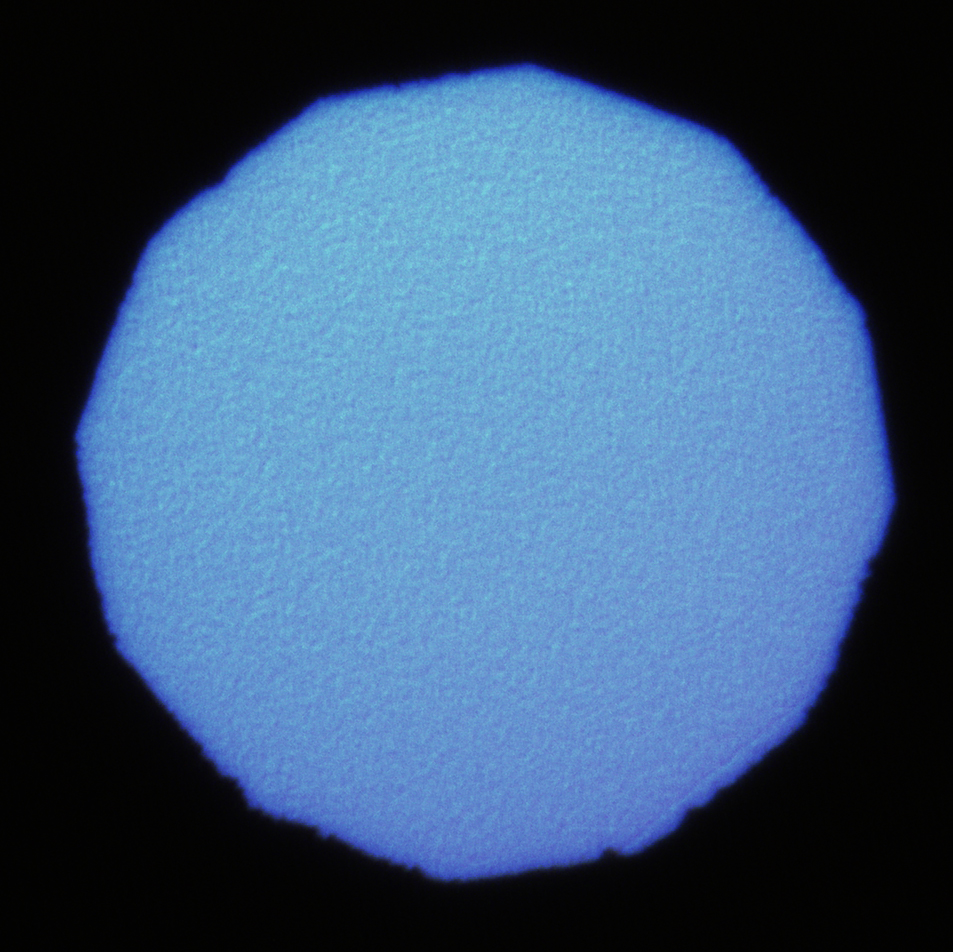
\includegraphics[totalheight=5 cm]{Grafiken/nix.jpg}\label{fig:nix}}\qquad
	\subfloat[]{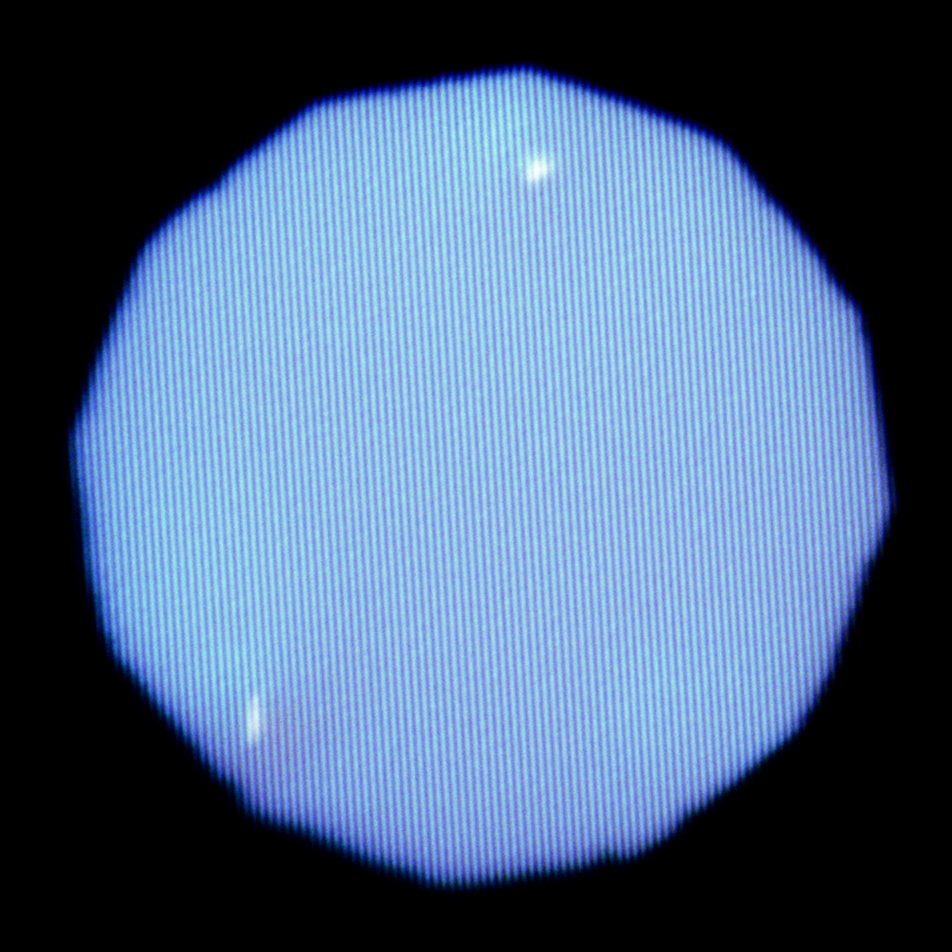
\includegraphics[totalheight=5 cm]{Grafiken/400nm.jpg} \label{fig:400nm}}\\%
%\end{adjustwidth}
\caption{Proben unter dem Lichtmikroskop. \textbf{(a)} Die Aufl�sung des Lichtmikroskops reicht nicht aus um die Strukturen aufzul�sen. \textbf{(b)} Gitterstruktur mit einer Periodizit�t von 400~nm.$^1$}%
\label{fig:matlab}%
\end{figure}

\begin{figure}%
\centering
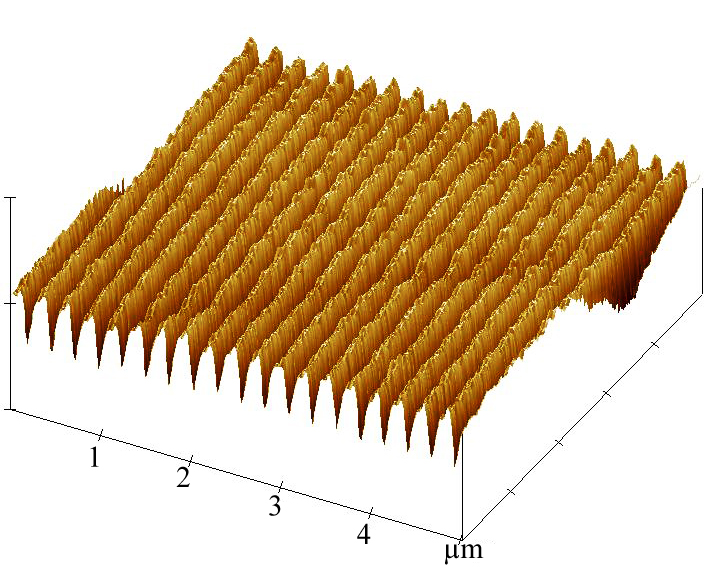
\includegraphics[width=.65\columnwidth]{Grafiken/3d_bild.jpg}%
\caption{AFM Messung der Topografie einer hergestellten Gitterstruktur (40~mJ, 4~s Entwicklungszeit).}%
\label{fig:3d_bild}%
\end{figure}


\section{Messung der Gitterperiode}

Aus den Aufgezeichneten H�henprofilen der Proben l�sst sich die Periodizit�t des hergestellten Gitters bestimmen. Abbildung \ref{fig:vgl_periode} zeigt das Profil zweier Proben. 
Zur Bestimmung der Periode wurden Zeiger auf zwei unterschiedlichen Maxima gesetzt. Die Software des AFMs gibt den Abstand beider Zeiger an. In Abbildung \ref{fig:periode1} betr�gt der Abstand beider schwarzen Zeiger 1,6~$\upmu$m und reicht �ber 6 Perioden. Damit ergibt sich f�r diese Probe eine Gitterperiode von 267~nm f�r die Probe mit einer Dosis von 40~mJ und einer Entwicklungszeit von 5~s.

Die Probe die mit einer Dosis von 20~mJ und einer Entwicklungszeit von 10~s hergestellt wurde (Abbildung \ref{fig:periode2}) hat ebenso eine Gitterperiode von 267~nm. Dies best�tigt \eqref{eq:periode}, dass die Gitterperiode nicht durch Belichtungsdosis oder Entwicklungszeit beeinflusst wird, sondern ma�geblich durch die Wellenl�nge bei der Laserinterferenzbelichtung bestimmt wird.

\begin{figure}[h]
\centering
%\begin{adjustwidth}{0cm}{0cm}
	\subfloat[40~mJ, 5~s]{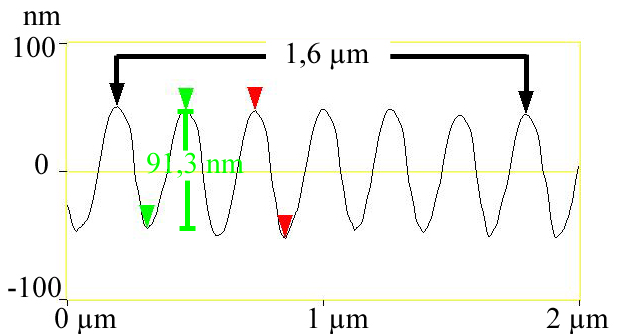
\includegraphics[totalheight=4 cm]{Grafiken/Periode_40mj_5s_1.jpg}\label{fig:periode1}}
	\subfloat[20~mJ, 10~s]{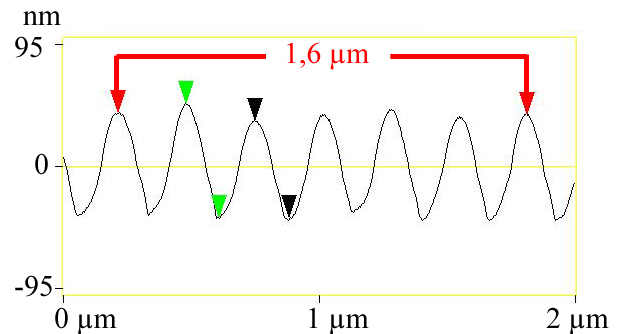
\includegraphics[totalheight=4 cm]{Grafiken/Periode_20mj_10s_w1.jpg} \label{fig:periode2}}
%\end{adjustwidth}
\caption{Mit dem AFM gemessene Gittertopographien. Gitterperiode beider Proben: $\sim$267~nm. \textbf{(a)} Dosis: 40~mJ, Entwicklungszeit: 5~s. \textbf{(b)} Dosis: 20~mJ, Entwicklungszeit 10~s. }%
\label{fig:vgl_periode}%
\end{figure}


\section{Messung der Gitteramplitude}

Weitergehend wurde anhand der Messungen die Gitteramplitude bestimmt. Hierzu wurden Zeiger einem Maximum und einem benachbarten Minimum gesetzt. Abbildung \ref{fig:periode1} zeigt einen H�henunterschied zwischen den gr�nen Zeigern von 91,3~nm. In jeder Messung wurde zum einen die maximale Amplitude als auch die minimale Amplitude bestimmt. 

Die Gitteramplitude zeigt eine starke Abh�ngigkeit von den Herstellungsparametern. Darum sollen im Folgenden die Auswirkungen der Belichtungsdosis und der Entwicklungszeit auf die hergestellten Gitterstrukturen untersucht werden. Hierzu werden neben den im Rahmen des Laborversuches hergestellten Proben (vgl. Tabelle \ref{tab:parameter}) auch weitere Proben verwendet. Diese wurden im Labor Nanotechnologie von Matthias Ba�ler, Simon Jau� und Martin Waldvogel unter Anleitung von Uwe Bog hergestellt und vermessen.\footnote[2]{Ba�ler, Jau�, Waldvogel; Pr�sentation zum Laboversuch Laser Interverenz Lithographie; 15.08.2011} Tabelle \ref{tab:Referenz} zeigt die Herstellungsparameter dieser Proben.

\begin{table}%
\centering
\caption{Von Laborgruppe ''Ba�ler``$^2$ hergestellte Proben.}
\begin{tabular}{cc}

\toprule
Entwicklungsdauer	& Belichtungsenergien\\
in s	& in mJ\\
\midrule
10 & 10, 40, 80\\
20  & 10, 40, 80\\
30 & 10, 40, 80\\
\bottomrule 
\end{tabular}
\label{tab:Referenz}
\end{table}

Zun�chst soll die Amplitude des Gitters in Abh�ngigkeit von der Strahlungsdosis untersucht werden. Hierzu wurde �ber alle Messwerte mit gleicher Belichtungszeit gemittelt. Diese Mittelwerte sind in Abbildung \ref{fig:Ampl1} aufgetragen. Man erkennt, dass die Gitteramplitude mit steigender Strahlungsdosis abnimmt. \todo{erkl�rung mit kontrastkurve veruchen}


\begin{figure}[h]
\centering
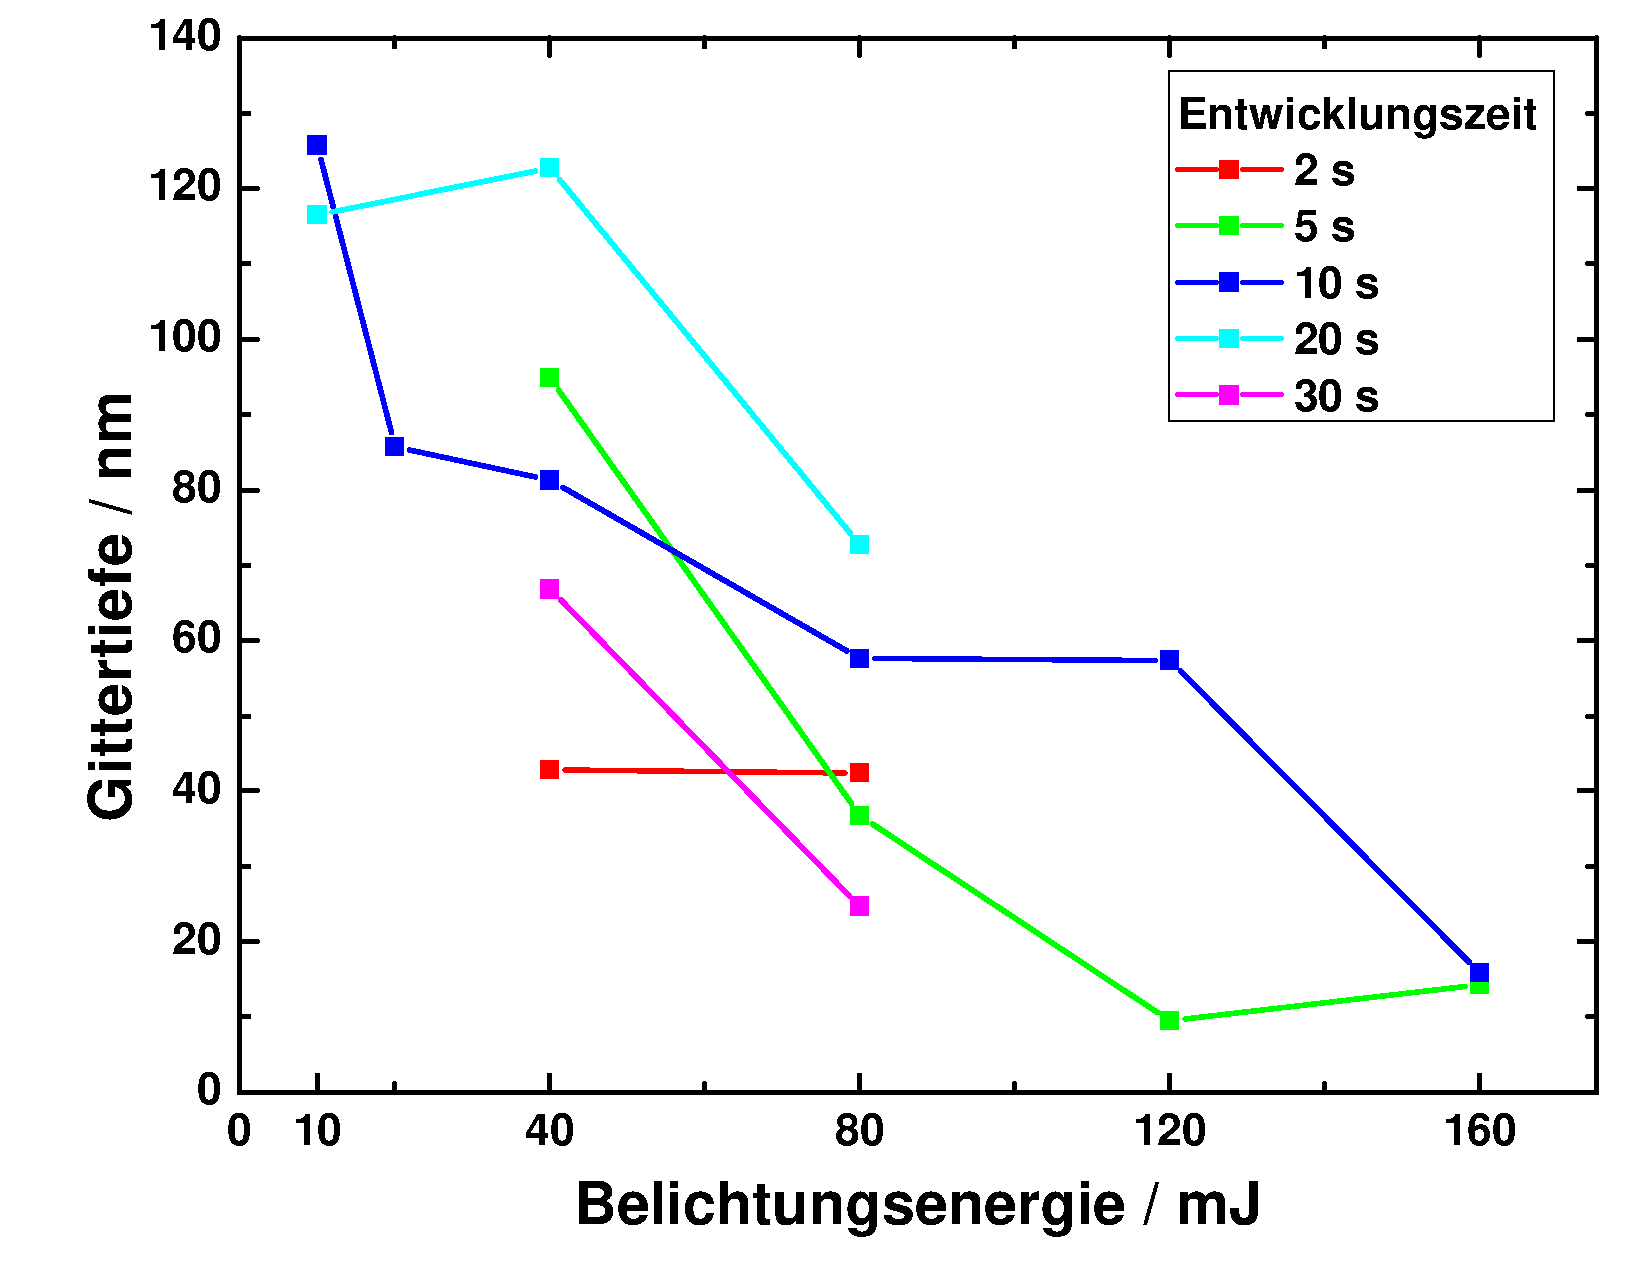
\includegraphics[width=.7\columnwidth]{Grafiken/Dosis.pdf}

\caption{}%
\label{fig:Ampl1}%
\end{figure}

\begin{figure}[h]
\centering
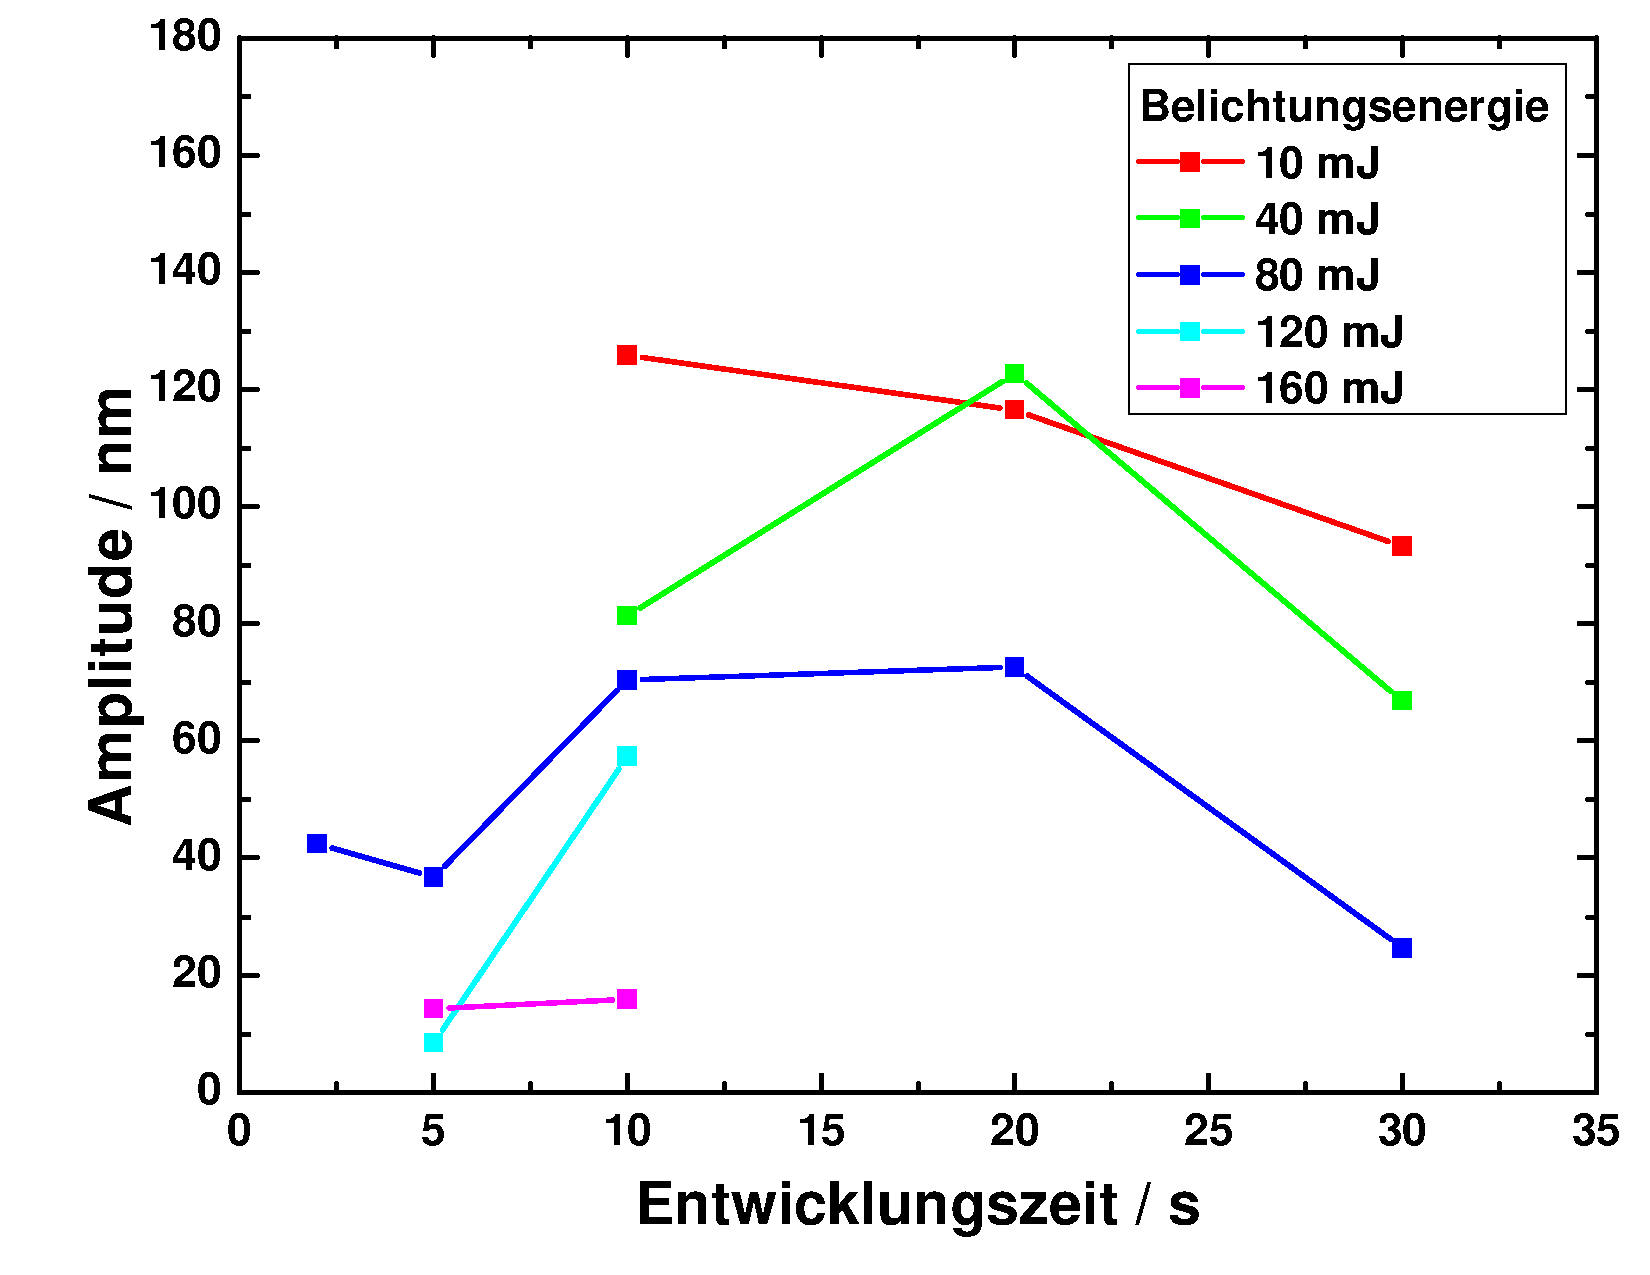
\includegraphics[width=.7\columnwidth]{Grafiken/Entwicklungszeit.pdf}
\caption{}%
\label{fig:Ampl2}%
\end{figure}

\section{Analyse der Gitterform}
